\documentclass{article}
\usepackage{dia-page}
\geometry{paperwidth=80mm, paperheight=92mm, vmargin=1pt, hmargin=1pt, nohead, nofoot}

\begin{document}

\centering

\begin{tikzpicture}[font=\diaSmall, node distance=2mm]
  \node (des) [font=\diaSmall] {\parbox{15mm}{\centering New desire}};

  \node (pur) [font=\diaSmall, below right=10mm and 30mm of des.mid, anchor=mid]
  {\parbox{18mm}{\centering Focusing on pursuit}};

  \node (ach) [font=\diaSmall, below right=25mm and 15mm of des.mid, anchor=mid]
  {\parbox{21mm}{\centering Achievement or failure}};

  \node (sat) [font=\diaSmall, below left=25mm and 15mm of des.mid, anchor=mid]
  {\parbox{21mm}{\centering Satisfied or disappointed}};

  \node (ada) [font=\diaSmall, below left=10mm and 30mm of des.mid, anchor=mid]
  {\parbox{19mm}{\centering Adapting the new as normal}};

  \draw [smallish arrow] (des) to (pur);
  \draw [smallish arrow] (pur) to (ach);
  \draw [smallish arrow] (ach) to (sat);
  \draw [smallish arrow] (sat) to (ada);
  \draw [smallish arrow] (ada) to (des);

  \node [below=35mm of des.south]
  {\parbox{70mm}{\centering 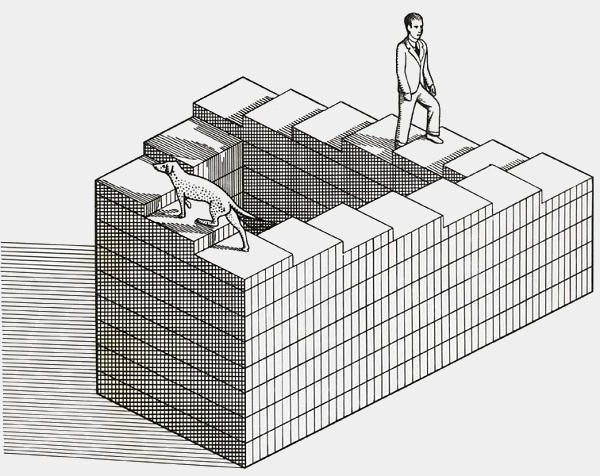
\includegraphics[width=60mm]{staircase-man-dog-flipped.jpg}}};

\end{tikzpicture}%

\end{document}
